\documentclass[1p]{elsarticle_modified}
%\bibliographystyle{elsarticle-num}

%\usepackage[colorlinks]{hyperref}
%\usepackage{abbrmath_seonhwa} %\Abb, \Ascr, \Acal ,\Abf, \Afrak
\usepackage{amsfonts}
\usepackage{amssymb}
\usepackage{amsmath}
\usepackage{amsthm}
\usepackage{scalefnt}
\usepackage{amsbsy}
\usepackage{kotex}
\usepackage{caption}
\usepackage{subfig}
\usepackage{color}
\usepackage{graphicx}
\usepackage{xcolor} %% white, black, red, green, blue, cyan, magenta, yellow
\usepackage{float}
\usepackage{setspace}
\usepackage{hyperref}

\usepackage{tikz}
\usetikzlibrary{arrows}

\usepackage{multirow}
\usepackage{array} % fixed length table
\usepackage{hhline}

%%%%%%%%%%%%%%%%%%%%%
\makeatletter
\renewcommand*\env@matrix[1][\arraystretch]{%
	\edef\arraystretch{#1}%
	\hskip -\arraycolsep
	\let\@ifnextchar\new@ifnextchar
	\array{*\c@MaxMatrixCols c}}
\makeatother %https://tex.stackexchange.com/questions/14071/how-can-i-increase-the-line-spacing-in-a-matrix
%%%%%%%%%%%%%%%

\usepackage[normalem]{ulem}

\newcommand{\msout}[1]{\ifmmode\text{\sout{\ensuremath{#1}}}\else\sout{#1}\fi}
%SOURCE: \msout is \stkout macro in https://tex.stackexchange.com/questions/20609/strikeout-in-math-mode

\newcommand{\cancel}[1]{
	\ifmmode
	{\color{red}\msout{#1}}
	\else
	{\color{red}\sout{#1}}
	\fi
}

\newcommand{\add}[1]{
	{\color{blue}\uwave{#1}}
}

\newcommand{\replace}[2]{
	\ifmmode
	{\color{red}\msout{#1}}{\color{blue}\uwave{#2}}
	\else
	{\color{red}\sout{#1}}{\color{blue}\uwave{#2}}
	\fi
}

\newcommand{\Sol}{\mathcal{S}} %segment
\newcommand{\D}{D} %diagram
\newcommand{\A}{\mathcal{A}} %arc


%%%%%%%%%%%%%%%%%%%%%%%%%%%%%5 test

\def\sl{\operatorname{\textup{SL}}(2,\Cbb)}
\def\psl{\operatorname{\textup{PSL}}(2,\Cbb)}
\def\quan{\mkern 1mu \triangleright \mkern 1mu}

\theoremstyle{definition}
\newtheorem{thm}{Theorem}[section]
\newtheorem{prop}[thm]{Proposition}
\newtheorem{lem}[thm]{Lemma}
\newtheorem{ques}[thm]{Question}
\newtheorem{cor}[thm]{Corollary}
\newtheorem{defn}[thm]{Definition}
\newtheorem{exam}[thm]{Example}
\newtheorem{rmk}[thm]{Remark}
\newtheorem{alg}[thm]{Algorithm}

\newcommand{\I}{\sqrt{-1}}
\begin{document}

%\begin{frontmatter}
%
%\title{Boundary parabolic representations of knots up to 8 crossings}
%
%%% Group authors per affiliation:
%\author{Yunhi Cho} 
%\address{Department of Mathematics, University of Seoul, Seoul, Korea}
%\ead{yhcho@uos.ac.kr}
%
%
%\author{Seonhwa Kim} %\fnref{s_kim}}
%\address{Center for Geometry and Physics, Institute for Basic Science, Pohang, 37673, Korea}
%\ead{ryeona17@ibs.re.kr}
%
%\author{Hyuk Kim}
%\address{Department of Mathematical Sciences, Seoul National University, Seoul 08826, Korea}
%\ead{hyukkim@snu.ac.kr}
%
%\author{Seokbeom Yoon}
%\address{Department of Mathematical Sciences, Seoul National University, Seoul, 08826,  Korea}
%\ead{sbyoon15@snu.ac.kr}
%
%\begin{abstract}
%We find all boundary parabolic representation of knots up to 8 crossings.
%
%\end{abstract}
%\begin{keyword}
%    \MSC[2010] 57M25 
%\end{keyword}
%
%\end{frontmatter}

%\linenumbers
%\tableofcontents
%
\newcommand\colored[1]{\textcolor{white}{\rule[-0.35ex]{0.8em}{1.4ex}}\kern-0.8em\color{red} #1}%
%\newcommand\colored[1]{\textcolor{white}{ #1}\kern-2.17ex	\textcolor{white}{ #1}\kern-1.81ex	\textcolor{white}{ #1}\kern-2.15ex\color{red}#1	}

{\Large $\underline{12n_{0315}~(K12n_{0315})}$}

\setlength{\tabcolsep}{10pt}
\renewcommand{\arraystretch}{1.6}
\vspace{1cm}\begin{tabular}{m{100pt}>{\centering\arraybackslash}m{274pt}}
\multirow{5}{120pt}{
	\centering
	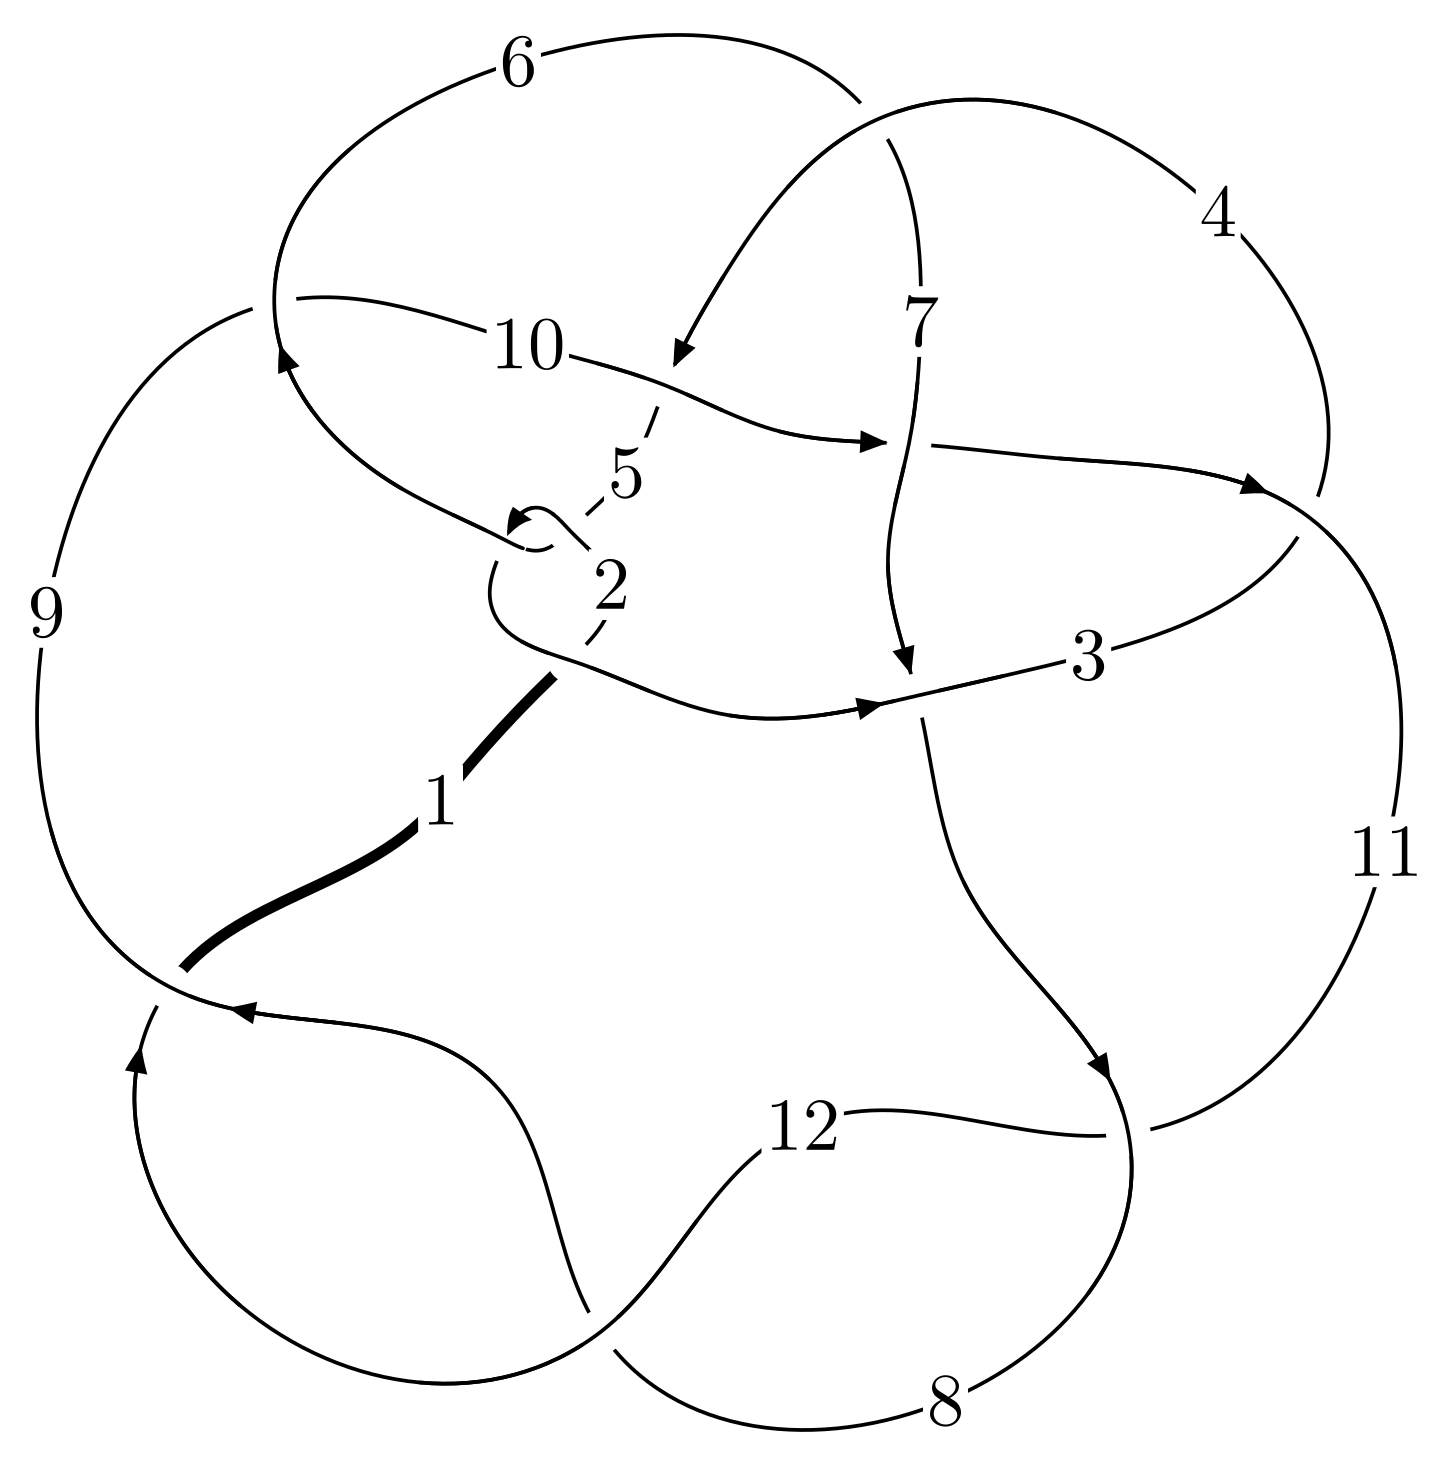
\includegraphics[width=112pt]{../../../GIT/diagram.site/Diagrams/png/2404_12n_0315.png}\\
\ \ \ A knot diagram\footnotemark}&
\allowdisplaybreaks
\textbf{Linearized knot diagam} \\
\cline{2-2}
 &
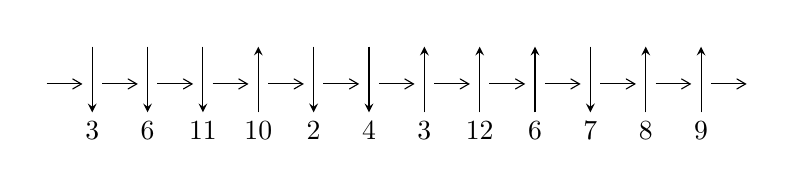
\begin{tikzpicture}[x=20pt, y=17pt]
	% nodes
	\node (C0) at (0, 0) {};
	\node (C1) at (1, 0) {};
	\node (C1U) at (1, +1) {};
	\node (C1D) at (1, -1) {3};

	\node (C2) at (2, 0) {};
	\node (C2U) at (2, +1) {};
	\node (C2D) at (2, -1) {6};

	\node (C3) at (3, 0) {};
	\node (C3U) at (3, +1) {};
	\node (C3D) at (3, -1) {11};

	\node (C4) at (4, 0) {};
	\node (C4U) at (4, +1) {};
	\node (C4D) at (4, -1) {10};

	\node (C5) at (5, 0) {};
	\node (C5U) at (5, +1) {};
	\node (C5D) at (5, -1) {2};

	\node (C6) at (6, 0) {};
	\node (C6U) at (6, +1) {};
	\node (C6D) at (6, -1) {4};

	\node (C7) at (7, 0) {};
	\node (C7U) at (7, +1) {};
	\node (C7D) at (7, -1) {3};

	\node (C8) at (8, 0) {};
	\node (C8U) at (8, +1) {};
	\node (C8D) at (8, -1) {12};

	\node (C9) at (9, 0) {};
	\node (C9U) at (9, +1) {};
	\node (C9D) at (9, -1) {6};

	\node (C10) at (10, 0) {};
	\node (C10U) at (10, +1) {};
	\node (C10D) at (10, -1) {7};

	\node (C11) at (11, 0) {};
	\node (C11U) at (11, +1) {};
	\node (C11D) at (11, -1) {8};

	\node (C12) at (12, 0) {};
	\node (C12U) at (12, +1) {};
	\node (C12D) at (12, -1) {9};
	\node (C13) at (13, 0) {};

	% arrows
	\draw[->,>={angle 60}]
	(C0) edge (C1) (C1) edge (C2) (C2) edge (C3) (C3) edge (C4) (C4) edge (C5) (C5) edge (C6) (C6) edge (C7) (C7) edge (C8) (C8) edge (C9) (C9) edge (C10) (C10) edge (C11) (C11) edge (C12) (C12) edge (C13) ;	\draw[->,>=stealth]
	(C1U) edge (C1D) (C2U) edge (C2D) (C3U) edge (C3D) (C4D) edge (C4U) (C5U) edge (C5D) (C6U) edge (C6D) (C7D) edge (C7U) (C8D) edge (C8U) (C9D) edge (C9U) (C10U) edge (C10D) (C11D) edge (C11U) (C12D) edge (C12U) ;
	\end{tikzpicture} \\
\hhline{~~} \\& 
\textbf{Solving Sequence} \\ \cline{2-2} 
 &
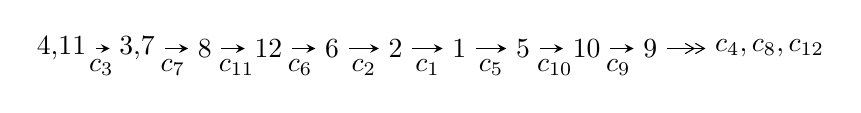
\begin{tikzpicture}[x=23pt, y=7pt]
	% node
	\node (A0) at (-1/8, 0) {4,11};
	\node (A1) at (17/16, 0) {3,7};
	\node (A2) at (17/8, 0) {8};
	\node (A3) at (25/8, 0) {12};
	\node (A4) at (33/8, 0) {6};
	\node (A5) at (41/8, 0) {2};
	\node (A6) at (49/8, 0) {1};
	\node (A7) at (57/8, 0) {5};
	\node (A8) at (65/8, 0) {10};
	\node (A9) at (73/8, 0) {9};
	\node (C1) at (1/2, -1) {$c_{3}$};
	\node (C2) at (13/8, -1) {$c_{7}$};
	\node (C3) at (21/8, -1) {$c_{11}$};
	\node (C4) at (29/8, -1) {$c_{6}$};
	\node (C5) at (37/8, -1) {$c_{2}$};
	\node (C6) at (45/8, -1) {$c_{1}$};
	\node (C7) at (53/8, -1) {$c_{5}$};
	\node (C8) at (61/8, -1) {$c_{10}$};
	\node (C9) at (69/8, -1) {$c_{9}$};
	\node (A10) at (11, 0) {$c_{4},c_{8},c_{12}$};

	% edge
	\draw[->,>=stealth]	
	(A0) edge (A1) (A1) edge (A2) (A2) edge (A3) (A3) edge (A4) (A4) edge (A5) (A5) edge (A6) (A6) edge (A7) (A7) edge (A8) (A8) edge (A9) ;
	\draw[->>,>={angle 60}]	
	(A9) edge (A10);
\end{tikzpicture} \\ 

\end{tabular} \\

\footnotetext{
The image of knot diagram is generated by the software ``\textbf{Draw programme}" developed by Andrew Bartholomew(\url{http://www.layer8.co.uk/maths/draw/index.htm\#Running-draw}), where we modified some parts for our purpose(\url{https://github.com/CATsTAILs/LinksPainter}).
}\phantom \\ \newline 
\centering \textbf{Ideals for irreducible components\footnotemark of $X_{\text{par}}$} 
 
\begin{align*}
I^u_{1}&=\langle 
1.20606\times10^{53} u^{43}-5.58942\times10^{53} u^{42}+\cdots+5.03135\times10^{53} b+2.95975\times10^{54},\\
\phantom{I^u_{1}}&\phantom{= \langle  }-3.18519\times10^{53} u^{43}-8.78761\times10^{54} u^{42}+\cdots+1.45909\times10^{55} a+5.45810\times10^{56},\\
\phantom{I^u_{1}}&\phantom{= \langle  }u^{44}-5 u^{43}+\cdots+42 u-29\rangle \\
I^u_{2}&=\langle 
- u^9+u^8- u^7+u^4+2 u^3- u^2+b+u,\;3 u^8-3 u^7+5 u^6-2 u^5+u^4-2 u^3-7 u^2+a+u-6,\\
\phantom{I^u_{2}}&\phantom{= \langle  }u^{10}- u^9+2 u^8- u^7+u^6- u^5-2 u^4-3 u^2-1\rangle \\
I^u_{3}&=\langle 
u^2+b+u,\;a,\;u^4+u^3+u^2+u+1\rangle \\
\\
\end{align*}
\raggedright * 3 irreducible components of $\dim_{\mathbb{C}}=0$, with total 58 representations.\\
\footnotetext{All coefficients of polynomials are rational numbers. But the coefficients are sometimes approximated in decimal forms when there is not enough margin.}
\newpage
\renewcommand{\arraystretch}{1}
\centering \section*{I. $I^u_{1}= \langle 1.21\times10^{53} u^{43}-5.59\times10^{53} u^{42}+\cdots+5.03\times10^{53} b+2.96\times10^{54},\;-3.19\times10^{53} u^{43}-8.79\times10^{54} u^{42}+\cdots+1.46\times10^{55} a+5.46\times10^{56},\;u^{44}-5 u^{43}+\cdots+42 u-29 \rangle$}
\flushleft \textbf{(i) Arc colorings}\\
\begin{tabular}{m{7pt} m{180pt} m{7pt} m{180pt} }
\flushright $a_{4}=$&$\begin{pmatrix}1\\0\end{pmatrix}$ \\
\flushright $a_{11}=$&$\begin{pmatrix}0\\u\end{pmatrix}$ \\
\flushright $a_{3}=$&$\begin{pmatrix}1\\- u^2\end{pmatrix}$ \\
\flushright $a_{7}=$&$\begin{pmatrix}0.0218300 u^{43}+0.602265 u^{42}+\cdots+35.6982 u-37.4075\\-0.239709 u^{43}+1.11092 u^{42}+\cdots+27.7492 u-5.88261\end{pmatrix}$ \\
\flushright $a_{8}=$&$\begin{pmatrix}0.116480 u^{43}-0.214561 u^{42}+\cdots+34.2011 u-22.6591\\0.196318 u^{43}-1.07204 u^{42}+\cdots+10.5743 u+4.08103\end{pmatrix}$ \\
\flushright $a_{12}=$&$\begin{pmatrix}-0.264193 u^{43}+0.881362 u^{42}+\cdots-44.3354 u+34.0722\\0.396645 u^{43}-2.17462 u^{42}+\cdots-57.8387 u+23.3029\end{pmatrix}$ \\
\flushright $a_{6}=$&$\begin{pmatrix}-0.217879 u^{43}+1.71318 u^{42}+\cdots+63.4475 u-43.2901\\-0.239709 u^{43}+1.11092 u^{42}+\cdots+27.7492 u-5.88261\end{pmatrix}$ \\
\flushright $a_{2}=$&$\begin{pmatrix}0.00263508 u^{43}-0.985931 u^{42}+\cdots-67.9139 u+53.2351\\0.161780 u^{43}-1.07286 u^{42}+\cdots-34.3822 u+20.2044\end{pmatrix}$ \\
\flushright $a_{1}=$&$\begin{pmatrix}-0.00400046 u^{43}-0.634908 u^{42}+\cdots-61.3639 u+45.2296\\-0.0666468 u^{43}+0.211695 u^{42}+\cdots-20.8403 u+10.9869\end{pmatrix}$ \\
\flushright $a_{5}=$&$\begin{pmatrix}-0.136976 u^{43}-1.16465 u^{42}+\cdots-39.2384 u+65.9737\\-0.0834339 u^{43}+0.546656 u^{42}+\cdots+17.1001 u-4.86412\end{pmatrix}$ \\
\flushright $a_{10}=$&$\begin{pmatrix}-1.27373 u^{43}+6.20997 u^{42}+\cdots+44.8550 u+10.4545\\-0.337820 u^{43}+1.39778 u^{42}+\cdots-9.87916 u+17.6646\end{pmatrix}$ \\
\flushright $a_{9}=$&$\begin{pmatrix}0.157901 u^{43}-1.21230 u^{42}+\cdots-74.0140 u+41.4809\\0.325629 u^{43}-1.96751 u^{42}+\cdots-60.8611 u+31.4254\end{pmatrix}$\\&\end{tabular}
\flushleft \textbf{(ii) Obstruction class $= -1$}\\~\\
\flushleft \textbf{(iii) Cusp Shapes $= 0.287876 u^{43}-2.76272 u^{42}+\cdots-100.619 u+56.2787$}\\~\\
\newpage\renewcommand{\arraystretch}{1}
\flushleft \textbf{(iv) u-Polynomials at the component}\newline \\
\begin{tabular}{m{50pt}|m{274pt}}
Crossings & \hspace{64pt}u-Polynomials at each crossing \\
\hline $$\begin{aligned}c_{1}\end{aligned}$$&$\begin{aligned}
&u^{44}+61 u^{43}+\cdots+654834 u+3025
\end{aligned}$\\
\hline $$\begin{aligned}c_{2},c_{5}\end{aligned}$$&$\begin{aligned}
&u^{44}+u^{43}+\cdots+592 u+55
\end{aligned}$\\
\hline $$\begin{aligned}c_{3}\end{aligned}$$&$\begin{aligned}
&u^{44}+5 u^{43}+\cdots-42 u-29
\end{aligned}$\\
\hline $$\begin{aligned}c_{4}\end{aligned}$$&$\begin{aligned}
&u^{44}+2 u^{43}+\cdots+583 u-121
\end{aligned}$\\
\hline $$\begin{aligned}c_{6}\end{aligned}$$&$\begin{aligned}
&u^{44}-6 u^{43}+\cdots+10 u-1
\end{aligned}$\\
\hline $$\begin{aligned}c_{7}\end{aligned}$$&$\begin{aligned}
&u^{44}- u^{43}+\cdots+295 u+229
\end{aligned}$\\
\hline $$\begin{aligned}c_{8},c_{11},c_{12}\end{aligned}$$&$\begin{aligned}
&u^{44}- u^{43}+\cdots-113 u-11
\end{aligned}$\\
\hline $$\begin{aligned}c_{9}\end{aligned}$$&$\begin{aligned}
&u^{44}+52 u^{42}+\cdots-10437016 u-496609
\end{aligned}$\\
\hline $$\begin{aligned}c_{10}\end{aligned}$$&$\begin{aligned}
&u^{44}+6 u^{43}+\cdots+248 u+80
\end{aligned}$\\
\hline
\end{tabular}\\~\\
\newpage\renewcommand{\arraystretch}{1}
\flushleft \textbf{(v) Riley Polynomials at the component}\newline \\
\begin{tabular}{m{50pt}|m{274pt}}
Crossings & \hspace{64pt}Riley Polynomials at each crossing \\
\hline $$\begin{aligned}c_{1}\end{aligned}$$&$\begin{aligned}
&y^{44}-157 y^{43}+\cdots-380470856606 y+9150625
\end{aligned}$\\
\hline $$\begin{aligned}c_{2},c_{5}\end{aligned}$$&$\begin{aligned}
&y^{44}-61 y^{43}+\cdots-654834 y+3025
\end{aligned}$\\
\hline $$\begin{aligned}c_{3}\end{aligned}$$&$\begin{aligned}
&y^{44}+13 y^{43}+\cdots+12678 y+841
\end{aligned}$\\
\hline $$\begin{aligned}c_{4}\end{aligned}$$&$\begin{aligned}
&y^{44}+52 y^{43}+\cdots-193721 y+14641
\end{aligned}$\\
\hline $$\begin{aligned}c_{6}\end{aligned}$$&$\begin{aligned}
&y^{44}+4 y^{43}+\cdots-18 y+1
\end{aligned}$\\
\hline $$\begin{aligned}c_{7}\end{aligned}$$&$\begin{aligned}
&y^{44}- y^{43}+\cdots-491439 y+52441
\end{aligned}$\\
\hline $$\begin{aligned}c_{8},c_{11},c_{12}\end{aligned}$$&$\begin{aligned}
&y^{44}-33 y^{43}+\cdots-24187 y+121
\end{aligned}$\\
\hline $$\begin{aligned}c_{9}\end{aligned}$$&$\begin{aligned}
&y^{44}+104 y^{43}+\cdots-91222464416576 y+246620498881
\end{aligned}$\\
\hline $$\begin{aligned}c_{10}\end{aligned}$$&$\begin{aligned}
&y^{44}-12 y^{43}+\cdots-113984 y+6400
\end{aligned}$\\
\hline
\end{tabular}\\~\\
\newpage\flushleft \textbf{(vi) Complex Volumes and Cusp Shapes}
$$\begin{array}{c|c|c}  
\text{Solutions to }I^u_{1}& \I (\text{vol} + \sqrt{-1}CS) & \text{Cusp shape}\\
 \hline 
\begin{aligned}
u &= -0.646694 + 0.709710 I \\
a &= -1.44530 - 0.26000 I \\
b &= \phantom{-}0.754661 - 1.033090 I\end{aligned}
 & -0.73884 + 3.57823 I & -2.03363 - 1.23509 I \\ \hline\begin{aligned}
u &= -0.646694 - 0.709710 I \\
a &= -1.44530 + 0.26000 I \\
b &= \phantom{-}0.754661 + 1.033090 I\end{aligned}
 & -0.73884 - 3.57823 I & -2.03363 + 1.23509 I \\ \hline\begin{aligned}
u &= \phantom{-}0.560756 + 0.906193 I \\
a &= \phantom{-}0.988565 - 0.382204 I \\
b &= -0.479339 - 0.355674 I\end{aligned}
 & -0.07583 - 2.23571 I & \phantom{-}0.15264 + 3.25000 I \\ \hline\begin{aligned}
u &= \phantom{-}0.560756 - 0.906193 I \\
a &= \phantom{-}0.988565 + 0.382204 I \\
b &= -0.479339 + 0.355674 I\end{aligned}
 & -0.07583 + 2.23571 I & \phantom{-}0.15264 - 3.25000 I \\ \hline\begin{aligned}
u &= -0.931877\phantom{ +0.000000I} \\
a &= \phantom{-}0.852980\phantom{ +0.000000I} \\
b &= -0.358962\phantom{ +0.000000I}\end{aligned}
 & \phantom{-}1.95891\phantom{ +0.000000I} & \phantom{-}7.69720\phantom{ +0.000000I} \\ \hline\begin{aligned}
u &= -0.134801 + 1.060870 I \\
a &= \phantom{-}0.326691 - 0.405578 I \\
b &= -0.036301 - 1.377150 I\end{aligned}
 & \phantom{-}8.47609 + 2.02964 I & \phantom{-}8.25034 - 3.54308 I \\ \hline\begin{aligned}
u &= -0.134801 - 1.060870 I \\
a &= \phantom{-}0.326691 + 0.405578 I \\
b &= -0.036301 + 1.377150 I\end{aligned}
 & \phantom{-}8.47609 - 2.02964 I & \phantom{-}8.25034 + 3.54308 I \\ \hline\begin{aligned}
u &= \phantom{-}0.494156 + 0.966731 I \\
a &= -0.87020 + 1.18836 I \\
b &= \phantom{-}0.641372 + 0.824984 I\end{aligned}
 & \phantom{-}0.09327 - 2.72034 I & \phantom{-}1.39183 + 2.41510 I \\ \hline\begin{aligned}
u &= \phantom{-}0.494156 - 0.966731 I \\
a &= -0.87020 - 1.18836 I \\
b &= \phantom{-}0.641372 - 0.824984 I\end{aligned}
 & \phantom{-}0.09327 + 2.72034 I & \phantom{-}1.39183 - 2.41510 I \\ \hline\begin{aligned}
u &= \phantom{-}0.229114 + 0.882547 I \\
a &= \phantom{-}2.27817 + 0.13416 I \\
b &= -1.118850 - 0.022452 I\end{aligned}
 & -4.56670 + 1.09587 I & -0.21127 + 1.60051 I\\
 \hline 
 \end{array}$$\newpage$$\begin{array}{c|c|c}  
\text{Solutions to }I^u_{1}& \I (\text{vol} + \sqrt{-1}CS) & \text{Cusp shape}\\
 \hline 
\begin{aligned}
u &= \phantom{-}0.229114 - 0.882547 I \\
a &= \phantom{-}2.27817 - 0.13416 I \\
b &= -1.118850 + 0.022452 I\end{aligned}
 & -4.56670 - 1.09587 I & -0.21127 - 1.60051 I \\ \hline\begin{aligned}
u &= \phantom{-}0.715929 + 0.820156 I \\
a &= \phantom{-}1.31822 - 0.95604 I \\
b &= -0.82920 - 1.28038 I\end{aligned}
 & -7.86621 - 0.05476 I & -0.99221 + 1.86582 I \\ \hline\begin{aligned}
u &= \phantom{-}0.715929 - 0.820156 I \\
a &= \phantom{-}1.31822 + 0.95604 I \\
b &= -0.82920 + 1.28038 I\end{aligned}
 & -7.86621 + 0.05476 I & -0.99221 - 1.86582 I \\ \hline\begin{aligned}
u &= \phantom{-}0.499429 + 0.740618 I \\
a &= -1.013390 + 0.171593 I \\
b &= \phantom{-}1.145160 - 0.547724 I\end{aligned}
 & -0.68618 - 1.34446 I & \phantom{-}1.50024 + 5.16811 I \\ \hline\begin{aligned}
u &= \phantom{-}0.499429 - 0.740618 I \\
a &= -1.013390 - 0.171593 I \\
b &= \phantom{-}1.145160 + 0.547724 I\end{aligned}
 & -0.68618 + 1.34446 I & \phantom{-}1.50024 - 5.16811 I \\ \hline\begin{aligned}
u &= \phantom{-}0.689773 + 0.925188 I \\
a &= \phantom{-}0.426003 - 0.482177 I \\
b &= -1.30573 + 1.09475 I\end{aligned}
 & -7.53216 - 5.34120 I & -0.67544 + 3.86207 I \\ \hline\begin{aligned}
u &= \phantom{-}0.689773 - 0.925188 I \\
a &= \phantom{-}0.426003 + 0.482177 I \\
b &= -1.30573 - 1.09475 I\end{aligned}
 & -7.53216 + 5.34120 I & -0.67544 - 3.86207 I \\ \hline\begin{aligned}
u &= \phantom{-}0.148274 + 0.828216 I \\
a &= -2.47783 - 1.74623 I \\
b &= -0.277976 + 0.017995 I\end{aligned}
 & -4.75567 - 2.81209 I & \phantom{-}2.57862 + 7.29704 I \\ \hline\begin{aligned}
u &= \phantom{-}0.148274 - 0.828216 I \\
a &= -2.47783 + 1.74623 I \\
b &= -0.277976 - 0.017995 I\end{aligned}
 & -4.75567 + 2.81209 I & \phantom{-}2.57862 - 7.29704 I \\ \hline\begin{aligned}
u &= -0.973154 + 0.747396 I \\
a &= \phantom{-}0.544042 + 0.618644 I \\
b &= -1.19354 - 0.90568 I\end{aligned}
 & -12.93820 - 0.76342 I & -3.80369 + 0. I\phantom{ +0.000000I}\\
 \hline 
 \end{array}$$\newpage$$\begin{array}{c|c|c}  
\text{Solutions to }I^u_{1}& \I (\text{vol} + \sqrt{-1}CS) & \text{Cusp shape}\\
 \hline 
\begin{aligned}
u &= -0.973154 - 0.747396 I \\
a &= \phantom{-}0.544042 - 0.618644 I \\
b &= -1.19354 + 0.90568 I\end{aligned}
 & -12.93820 + 0.76342 I & -3.80369 + 0. I\phantom{ +0.000000I} \\ \hline\begin{aligned}
u &= -0.519846 + 1.144310 I \\
a &= -1.36543 - 0.79561 I \\
b &= \phantom{-}0.887391 - 0.816016 I\end{aligned}
 & \phantom{-}0.76786 + 6.70478 I & \phantom{-0.000000 } 0. - 7.25034 I \\ \hline\begin{aligned}
u &= -0.519846 - 1.144310 I \\
a &= -1.36543 + 0.79561 I \\
b &= \phantom{-}0.887391 + 0.816016 I\end{aligned}
 & \phantom{-}0.76786 - 6.70478 I & \phantom{-0.000000 -}0. + 7.25034 I \\ \hline\begin{aligned}
u &= -0.676167 + 0.306109 I \\
a &= -1.147500 - 0.672697 I \\
b &= \phantom{-}0.803888 + 0.651455 I\end{aligned}
 & -1.75012 - 2.06472 I & -2.87061 + 3.92303 I \\ \hline\begin{aligned}
u &= -0.676167 - 0.306109 I \\
a &= -1.147500 + 0.672697 I \\
b &= \phantom{-}0.803888 - 0.651455 I\end{aligned}
 & -1.75012 + 2.06472 I & -2.87061 - 3.92303 I \\ \hline\begin{aligned}
u &= \phantom{-}1.191210 + 0.490115 I \\
a &= \phantom{-}0.654463 - 0.667822 I \\
b &= -1.082710 + 0.775736 I\end{aligned}
 & -9.49734 + 7.11306 I & \phantom{-0.000000 } 0 \\ \hline\begin{aligned}
u &= \phantom{-}1.191210 - 0.490115 I \\
a &= \phantom{-}0.654463 + 0.667822 I \\
b &= -1.082710 - 0.775736 I\end{aligned}
 & -9.49734 - 7.11306 I & \phantom{-0.000000 } 0 \\ \hline\begin{aligned}
u &= -0.605021 + 1.146520 I \\
a &= \phantom{-}1.059940 + 0.253544 I \\
b &= -0.731247 + 0.441154 I\end{aligned}
 & \phantom{-}4.82729 + 5.41905 I & \phantom{-0.000000 } 0 \\ \hline\begin{aligned}
u &= -0.605021 - 1.146520 I \\
a &= \phantom{-}1.059940 - 0.253544 I \\
b &= -0.731247 - 0.441154 I\end{aligned}
 & \phantom{-}4.82729 - 5.41905 I & \phantom{-0.000000 } 0 \\ \hline\begin{aligned}
u &= -0.103748 + 0.684443 I \\
a &= \phantom{-}1.224370 + 0.560955 I \\
b &= -0.043528 + 0.580499 I\end{aligned}
 & \phantom{-}1.21862 - 0.91087 I & \phantom{-}6.00533 + 4.55629 I\\
 \hline 
 \end{array}$$\newpage$$\begin{array}{c|c|c}  
\text{Solutions to }I^u_{1}& \I (\text{vol} + \sqrt{-1}CS) & \text{Cusp shape}\\
 \hline 
\begin{aligned}
u &= -0.103748 - 0.684443 I \\
a &= \phantom{-}1.224370 - 0.560955 I \\
b &= -0.043528 - 0.580499 I\end{aligned}
 & \phantom{-}1.21862 + 0.91087 I & \phantom{-}6.00533 - 4.55629 I \\ \hline\begin{aligned}
u &= \phantom{-}0.679096\phantom{ +0.000000I} \\
a &= -0.424824\phantom{ +0.000000I} \\
b &= \phantom{-}0.727825\phantom{ +0.000000I}\end{aligned}
 & -1.43381\phantom{ +0.000000I} & -8.35220\phantom{ +0.000000I} \\ \hline\begin{aligned}
u &= -0.806563 + 1.049120 I \\
a &= \phantom{-}1.29333 + 0.62058 I \\
b &= -1.01794 + 1.20383 I\end{aligned}
 & -11.95870 + 7.26271 I & \phantom{-0.000000 } 0 \\ \hline\begin{aligned}
u &= -0.806563 - 1.049120 I \\
a &= \phantom{-}1.29333 - 0.62058 I \\
b &= -1.01794 - 1.20383 I\end{aligned}
 & -11.95870 - 7.26271 I & \phantom{-0.000000 } 0 \\ \hline\begin{aligned}
u &= -0.042706 + 0.623007 I \\
a &= -0.75781 + 1.69326 I \\
b &= \phantom{-}0.35910 + 1.52836 I\end{aligned}
 & \phantom{-}6.53095 - 1.24141 I & \phantom{-}1.101277 + 0.846650 I \\ \hline\begin{aligned}
u &= -0.042706 - 0.623007 I \\
a &= -0.75781 - 1.69326 I \\
b &= \phantom{-}0.35910 - 1.52836 I\end{aligned}
 & \phantom{-}6.53095 + 1.24141 I & \phantom{-}1.101277 - 0.846650 I \\ \hline\begin{aligned}
u &= \phantom{-}0.827601 + 1.122030 I \\
a &= -1.017800 + 0.089758 I \\
b &= \phantom{-}0.781744 + 1.041420 I\end{aligned}
 & \phantom{-}0.99079 - 7.76049 I & \phantom{-0.000000 } 0 \\ \hline\begin{aligned}
u &= \phantom{-}0.827601 - 1.122030 I \\
a &= -1.017800 - 0.089758 I \\
b &= \phantom{-}0.781744 - 1.041420 I\end{aligned}
 & \phantom{-}0.99079 + 7.76049 I & \phantom{-0.000000 } 0 \\ \hline\begin{aligned}
u &= -0.69348 + 1.23762 I \\
a &= -0.128890 - 0.232242 I \\
b &= \phantom{-}0.593220 + 0.522980 I\end{aligned}
 & \phantom{-}0.81092 + 1.60255 I & \phantom{-0.000000 } 0 \\ \hline\begin{aligned}
u &= -0.69348 - 1.23762 I \\
a &= -0.128890 + 0.232242 I \\
b &= \phantom{-}0.593220 - 0.522980 I\end{aligned}
 & \phantom{-}0.81092 - 1.60255 I & \phantom{-0.000000 } 0\\
 \hline 
 \end{array}$$\newpage$$\begin{array}{c|c|c}  
\text{Solutions to }I^u_{1}& \I (\text{vol} + \sqrt{-1}CS) & \text{Cusp shape}\\
 \hline 
\begin{aligned}
u &= \phantom{-}0.76866 + 1.22958 I \\
a &= \phantom{-}1.209600 - 0.452753 I \\
b &= -1.12581 - 1.15829 I\end{aligned}
 & -7.1426 - 14.0288 I & \phantom{-0.000000 } 0 \\ \hline\begin{aligned}
u &= \phantom{-}0.76866 - 1.22958 I \\
a &= \phantom{-}1.209600 + 0.452753 I \\
b &= -1.12581 + 1.15829 I\end{aligned}
 & -7.1426 + 14.0288 I & \phantom{-0.000000 } 0 \\ \hline\begin{aligned}
u &= \phantom{-}1.70367 + 1.24530 I \\
a &= \phantom{-}0.0487407 + 0.1311720 I \\
b &= \phantom{-}0.091200 - 0.327127 I\end{aligned}
 & -0.527893 + 0.187966 I & \phantom{-0.000000 } 0 \\ \hline\begin{aligned}
u &= \phantom{-}1.70367 - 1.24530 I \\
a &= \phantom{-}0.0487407 - 0.1311720 I \\
b &= \phantom{-}0.091200 + 0.327127 I\end{aligned}
 & -0.527893 - 0.187966 I & \phantom{-0.000000 } 0\\
 \hline 
 \end{array}$$\newpage\newpage\renewcommand{\arraystretch}{1}
\centering \section*{II. $I^u_{2}= \langle - u^9+u^8- u^7+u^4+2 u^3- u^2+b+u,\;3 u^8-3 u^7+\cdots+a-6,\;u^{10}- u^9+2 u^8- u^7+u^6- u^5-2 u^4-3 u^2-1 \rangle$}
\flushleft \textbf{(i) Arc colorings}\\
\begin{tabular}{m{7pt} m{180pt} m{7pt} m{180pt} }
\flushright $a_{4}=$&$\begin{pmatrix}1\\0\end{pmatrix}$ \\
\flushright $a_{11}=$&$\begin{pmatrix}0\\u\end{pmatrix}$ \\
\flushright $a_{3}=$&$\begin{pmatrix}1\\- u^2\end{pmatrix}$ \\
\flushright $a_{7}=$&$\begin{pmatrix}-3 u^8+3 u^7-5 u^6+2 u^5- u^4+2 u^3+7 u^2- u+6\\u^9- u^8+u^7- u^4-2 u^3+u^2- u\end{pmatrix}$ \\
\flushright $a_{8}=$&$\begin{pmatrix}u^9-3 u^8+3 u^7-3 u^6+u^5- u^4- u^3+5 u^2-2 u+3\\2 u^9-2 u^8+2 u^7- u^4-4 u^3+u^2-2 u-1\end{pmatrix}$ \\
\flushright $a_{12}=$&$\begin{pmatrix}u^7- u^6+u^5- u^2-2 u+1\\u^9+u^7+u^6-3 u^3-3 u^2-3 u-3\end{pmatrix}$ \\
\flushright $a_{6}=$&$\begin{pmatrix}u^9-4 u^8+4 u^7-5 u^6+2 u^5-2 u^4+8 u^2-2 u+6\\u^9- u^8+u^7- u^4-2 u^3+u^2- u\end{pmatrix}$ \\
\flushright $a_{2}=$&$\begin{pmatrix}2 u^9-8 u^8+9 u^7-10 u^6+4 u^5-3 u^4+14 u^2-6 u+11\\u^9- u^8+u^7- u^4-2 u^3- u-1\end{pmatrix}$ \\
\flushright $a_{1}=$&$\begin{pmatrix}2 u^9-5 u^8+6 u^7-5 u^6+2 u^5-2 u^4-2 u^3+7 u^2-5 u+4\\u^9+2 u^6- u^5-3 u^3-2 u^2- u-4\end{pmatrix}$ \\
\flushright $a_{5}=$&$\begin{pmatrix}-5 u^9+13 u^8-17 u^7+15 u^6-6 u^5+5 u^4+5 u^3-17 u^2+16 u-13\\- u^8+u^7-2 u^6+u^5- u^4+u^3+2 u^2+3\end{pmatrix}$ \\
\flushright $a_{10}=$&$\begin{pmatrix}-8 u^9+7 u^8-10 u^7+u^6+5 u^4+17 u^3- u^2+14 u+5\\u^9- u^8+2 u^7- u^6+u^5- u^4-2 u^3-3 u\end{pmatrix}$ \\
\flushright $a_{9}=$&$\begin{pmatrix}2 u^9+2 u^7+u^6- u^4-6 u^3-4 u^2-5 u-3\\- u^9+3 u^8-3 u^7+3 u^6- u^5+u^4+u^3-5 u^2+2 u-3\end{pmatrix}$\\&\end{tabular}
\flushleft \textbf{(ii) Obstruction class $= 1$}\\~\\
\flushleft \textbf{(iii) Cusp Shapes $= 4 u^9- u^8+u^7+3 u^6-2 u^5-5 u^4-11 u^3-2 u^2-4 u-3$}\\~\\
\newpage\renewcommand{\arraystretch}{1}
\flushleft \textbf{(iv) u-Polynomials at the component}\newline \\
\begin{tabular}{m{50pt}|m{274pt}}
Crossings & \hspace{64pt}u-Polynomials at each crossing \\
\hline $$\begin{aligned}c_{1}\end{aligned}$$&$\begin{aligned}
&u^{10}-10 u^9+37 u^8-58 u^7+70 u^6-51 u^5+29 u^4-27 u^3+4 u^2- u+1
\end{aligned}$\\
\hline $$\begin{aligned}c_{2}\end{aligned}$$&$\begin{aligned}
&u^{10}+6 u^9+13 u^8+10 u^7-6 u^6-19 u^5-15 u^4-3 u^3+4 u^2+3 u+1
\end{aligned}$\\
\hline $$\begin{aligned}c_{3}\end{aligned}$$&$\begin{aligned}
&u^{10}- u^9+2 u^8- u^7+u^6- u^5-2 u^4-3 u^2-1
\end{aligned}$\\
\hline $$\begin{aligned}c_{4}\end{aligned}$$&$\begin{aligned}
&u^{10}+3 u^8+2 u^6+u^5- u^4+u^3-2 u^2+u-1
\end{aligned}$\\
\hline $$\begin{aligned}c_{5}\end{aligned}$$&$\begin{aligned}
&u^{10}-6 u^9+13 u^8-10 u^7-6 u^6+19 u^5-15 u^4+3 u^3+4 u^2-3 u+1
\end{aligned}$\\
\hline $$\begin{aligned}c_{6}\end{aligned}$$&$\begin{aligned}
&u^{10}+3 u^9+6 u^8+7 u^7+4 u^6-3 u^5-6 u^4-2 u^3+4 u^2+4 u+1
\end{aligned}$\\
\hline $$\begin{aligned}c_{7}\end{aligned}$$&$\begin{aligned}
&u^{10}-7 u^8-12 u^7+16 u^6+40 u^5+27 u^4- u^3+u-1
\end{aligned}$\\
\hline $$\begin{aligned}c_{8}\end{aligned}$$&$\begin{aligned}
&u^{10}-6 u^8+2 u^7+13 u^6-8 u^5-11 u^4+9 u^3+2 u^2-2 u+1
\end{aligned}$\\
\hline $$\begin{aligned}c_{9}\end{aligned}$$&$\begin{aligned}
&u^{10}+u^9+15 u^8+37 u^6+16 u^4-9 u^3-8 u^2- u+1
\end{aligned}$\\
\hline $$\begin{aligned}c_{10}\end{aligned}$$&$\begin{aligned}
&u^{10}- u^9+2 u^8-11 u^7+16 u^6+6 u^5-17 u^4-51 u^3+104 u^2-53 u+5
\end{aligned}$\\
\hline $$\begin{aligned}c_{11},c_{12}\end{aligned}$$&$\begin{aligned}
&u^{10}-6 u^8-2 u^7+13 u^6+8 u^5-11 u^4-9 u^3+2 u^2+2 u+1
\end{aligned}$\\
\hline
\end{tabular}\\~\\
\newpage\renewcommand{\arraystretch}{1}
\flushleft \textbf{(v) Riley Polynomials at the component}\newline \\
\begin{tabular}{m{50pt}|m{274pt}}
Crossings & \hspace{64pt}Riley Polynomials at each crossing \\
\hline $$\begin{aligned}c_{1}\end{aligned}$$&$\begin{aligned}
&y^{10}-26 y^9+\cdots+7 y+1
\end{aligned}$\\
\hline $$\begin{aligned}c_{2},c_{5}\end{aligned}$$&$\begin{aligned}
&y^{10}-10 y^9+37 y^8-58 y^7+70 y^6-51 y^5+29 y^4-27 y^3+4 y^2- y+1
\end{aligned}$\\
\hline $$\begin{aligned}c_{3}\end{aligned}$$&$\begin{aligned}
&y^{10}+3 y^9+4 y^8-3 y^7-15 y^6-19 y^5-6 y^4+10 y^3+13 y^2+6 y+1
\end{aligned}$\\
\hline $$\begin{aligned}c_{4}\end{aligned}$$&$\begin{aligned}
&y^{10}+6 y^9+13 y^8+10 y^7-6 y^6-19 y^5-15 y^4-3 y^3+4 y^2+3 y+1
\end{aligned}$\\
\hline $$\begin{aligned}c_{6}\end{aligned}$$&$\begin{aligned}
&y^{10}+3 y^9+2 y^8+5 y^7+6 y^6-3 y^5+12 y^4-20 y^3+20 y^2-8 y+1
\end{aligned}$\\
\hline $$\begin{aligned}c_{7}\end{aligned}$$&$\begin{aligned}
&y^{10}-14 y^9+\cdots- y+1
\end{aligned}$\\
\hline $$\begin{aligned}c_{8},c_{11},c_{12}\end{aligned}$$&$\begin{aligned}
&y^{10}-12 y^9+\cdots+18 y^2+1
\end{aligned}$\\
\hline $$\begin{aligned}c_{9}\end{aligned}$$&$\begin{aligned}
&y^{10}+29 y^9+\cdots-17 y+1
\end{aligned}$\\
\hline $$\begin{aligned}c_{10}\end{aligned}$$&$\begin{aligned}
&y^{10}+3 y^9+\cdots-1769 y+25
\end{aligned}$\\
\hline
\end{tabular}\\~\\
\newpage\flushleft \textbf{(vi) Complex Volumes and Cusp Shapes}
$$\begin{array}{c|c|c}  
\text{Solutions to }I^u_{2}& \I (\text{vol} + \sqrt{-1}CS) & \text{Cusp shape}\\
 \hline 
\begin{aligned}
u &= -0.970948\phantom{ +0.000000I} \\
a &= \phantom{-}0.125163\phantom{ +0.000000I} \\
b &= \phantom{-}0.485263\phantom{ +0.000000I}\end{aligned}
 & -0.629142\phantom{ +0.000000I} & \phantom{-}4.19170\phantom{ +0.000000I} \\ \hline\begin{aligned}
u &= \phantom{-}0.275604 + 0.891818 I \\
a &= -0.521340 + 1.227210 I \\
b &= \phantom{-}0.12415 + 1.53429 I\end{aligned}
 & \phantom{-}6.96867 - 2.45082 I & \phantom{-}2.80943 + 5.14150 I \\ \hline\begin{aligned}
u &= \phantom{-}0.275604 - 0.891818 I \\
a &= -0.521340 - 1.227210 I \\
b &= \phantom{-}0.12415 - 1.53429 I\end{aligned}
 & \phantom{-}6.96867 + 2.45082 I & \phantom{-}2.80943 - 5.14150 I \\ \hline\begin{aligned}
u &= -0.488238 + 0.958609 I \\
a &= -1.23025 - 0.71023 I \\
b &= \phantom{-}0.673452 - 0.956870 I\end{aligned}
 & \phantom{-}0.20069 + 4.40188 I & \phantom{-}3.38083 - 6.40382 I \\ \hline\begin{aligned}
u &= -0.488238 - 0.958609 I \\
a &= -1.23025 + 0.71023 I \\
b &= \phantom{-}0.673452 + 0.956870 I\end{aligned}
 & \phantom{-}0.20069 - 4.40188 I & \phantom{-}3.38083 + 6.40382 I \\ \hline\begin{aligned}
u &= \phantom{-}1.26392\phantom{ +0.000000I} \\
a &= -0.608152\phantom{ +0.000000I} \\
b &= \phantom{-}0.615015\phantom{ +0.000000I}\end{aligned}
 & \phantom{-}1.41391\phantom{ +0.000000I} & -8.87500\phantom{ +0.000000I} \\ \hline\begin{aligned}
u &= \phantom{-}0.634722 + 1.144960 I \\
a &= -1.149300 + 0.305987 I \\
b &= \phantom{-}0.956654 + 0.685271 I\end{aligned}
 & \phantom{-}4.21151 - 6.16726 I & \phantom{-}1.23716 + 7.09016 I \\ \hline\begin{aligned}
u &= \phantom{-}0.634722 - 1.144960 I \\
a &= -1.149300 - 0.305987 I \\
b &= \phantom{-}0.956654 - 0.685271 I\end{aligned}
 & \phantom{-}4.21151 + 6.16726 I & \phantom{-}1.23716 - 7.09016 I \\ \hline\begin{aligned}
u &= -0.068575 + 0.683246 I \\
a &= \phantom{-}3.14239 - 1.75200 I \\
b &= -0.804393 - 0.314356 I\end{aligned}
 & -5.19351 + 2.25286 I & -4.08574 - 0.02786 I \\ \hline\begin{aligned}
u &= -0.068575 - 0.683246 I \\
a &= \phantom{-}3.14239 + 1.75200 I \\
b &= -0.804393 + 0.314356 I\end{aligned}
 & -5.19351 - 2.25286 I & -4.08574 + 0.02786 I\\
 \hline 
 \end{array}$$\newpage\newpage\renewcommand{\arraystretch}{1}
\centering \section*{III. $I^u_{3}= \langle u^2+b+u,\;a,\;u^4+u^3+u^2+u+1 \rangle$}
\flushleft \textbf{(i) Arc colorings}\\
\begin{tabular}{m{7pt} m{180pt} m{7pt} m{180pt} }
\flushright $a_{4}=$&$\begin{pmatrix}1\\0\end{pmatrix}$ \\
\flushright $a_{11}=$&$\begin{pmatrix}0\\u\end{pmatrix}$ \\
\flushright $a_{3}=$&$\begin{pmatrix}1\\- u^2\end{pmatrix}$ \\
\flushright $a_{7}=$&$\begin{pmatrix}0\\- u^2- u\end{pmatrix}$ \\
\flushright $a_{8}=$&$\begin{pmatrix}- u^2- u\\-2 u^2-2 u-1\end{pmatrix}$ \\
\flushright $a_{12}=$&$\begin{pmatrix}- u^3-2 u^2-2 u-1\\- u^3-3 u^2-3 u-2\end{pmatrix}$ \\
\flushright $a_{6}=$&$\begin{pmatrix}- u^2- u\\- u^2- u\end{pmatrix}$ \\
\flushright $a_{2}=$&$\begin{pmatrix}u^2+u+1\\u\end{pmatrix}$ \\
\flushright $a_{1}=$&$\begin{pmatrix}u^2+u\\u^2+u\end{pmatrix}$ \\
\flushright $a_{5}=$&$\begin{pmatrix}1\\- u^2\end{pmatrix}$ \\
\flushright $a_{10}=$&$\begin{pmatrix}0\\u\end{pmatrix}$ \\
\flushright $a_{9}=$&$\begin{pmatrix}u^3+2 u^2+2 u+1\\u^3+2 u^2+3 u+1\end{pmatrix}$\\&\end{tabular}
\flushleft \textbf{(ii) Obstruction class $= 1$}\\~\\
\flushleft \textbf{(iii) Cusp Shapes $= -2 u^3+u+1$}\\~\\
\newpage\renewcommand{\arraystretch}{1}
\flushleft \textbf{(iv) u-Polynomials at the component}\newline \\
\begin{tabular}{m{50pt}|m{274pt}}
Crossings & \hspace{64pt}u-Polynomials at each crossing \\
\hline $$\begin{aligned}c_{1},c_{2}\end{aligned}$$&$\begin{aligned}
&(u-1)^4
\end{aligned}$\\
\hline $$\begin{aligned}c_{3},c_{4}\end{aligned}$$&$\begin{aligned}
&u^4+u^3+u^2+u+1
\end{aligned}$\\
\hline $$\begin{aligned}c_{5}\end{aligned}$$&$\begin{aligned}
&(u+1)^4
\end{aligned}$\\
\hline $$\begin{aligned}c_{6},c_{7}\end{aligned}$$&$\begin{aligned}
&u^4+2 u^3+4 u^2+3 u+1
\end{aligned}$\\
\hline $$\begin{aligned}c_{8}\end{aligned}$$&$\begin{aligned}
&(u^2- u-1)^2
\end{aligned}$\\
\hline $$\begin{aligned}c_{9},c_{11},c_{12}\end{aligned}$$&$\begin{aligned}
&(u^2+u-1)^2
\end{aligned}$\\
\hline $$\begin{aligned}c_{10}\end{aligned}$$&$\begin{aligned}
&u^4
\end{aligned}$\\
\hline
\end{tabular}\\~\\
\newpage\renewcommand{\arraystretch}{1}
\flushleft \textbf{(v) Riley Polynomials at the component}\newline \\
\begin{tabular}{m{50pt}|m{274pt}}
Crossings & \hspace{64pt}Riley Polynomials at each crossing \\
\hline $$\begin{aligned}c_{1},c_{2},c_{5}\end{aligned}$$&$\begin{aligned}
&(y-1)^4
\end{aligned}$\\
\hline $$\begin{aligned}c_{3},c_{4}\end{aligned}$$&$\begin{aligned}
&y^4+y^3+y^2+y+1
\end{aligned}$\\
\hline $$\begin{aligned}c_{6},c_{7}\end{aligned}$$&$\begin{aligned}
&y^4+4 y^3+6 y^2- y+1
\end{aligned}$\\
\hline $$\begin{aligned}c_{8},c_{9},c_{11}\\c_{12}\end{aligned}$$&$\begin{aligned}
&(y^2-3 y+1)^2
\end{aligned}$\\
\hline $$\begin{aligned}c_{10}\end{aligned}$$&$\begin{aligned}
&y^4
\end{aligned}$\\
\hline
\end{tabular}\\~\\
\newpage\flushleft \textbf{(vi) Complex Volumes and Cusp Shapes}
$$\begin{array}{c|c|c}  
\text{Solutions to }I^u_{3}& \I (\text{vol} + \sqrt{-1}CS) & \text{Cusp shape}\\
 \hline 
\begin{aligned}
u &= \phantom{-}0.309017 + 0.951057 I \\
a &= \phantom{-0.000000 } 0 \\
b &= \phantom{-}0.50000 - 1.53884 I\end{aligned}
 & \phantom{-}7.23771\phantom{ +0.000000I} & \phantom{-}2.92705 + 2.12663 I \\ \hline\begin{aligned}
u &= \phantom{-}0.309017 - 0.951057 I \\
a &= \phantom{-0.000000 } 0 \\
b &= \phantom{-}0.50000 + 1.53884 I\end{aligned}
 & \phantom{-}7.23771\phantom{ +0.000000I} & \phantom{-}2.92705 - 2.12663 I \\ \hline\begin{aligned}
u &= -0.809017 + 0.587785 I \\
a &= \phantom{-0.000000 } 0 \\
b &= \phantom{-}0.500000 + 0.363271 I\end{aligned}
 & -0.657974\phantom{ +0.000000I} & -0.427051 - 1.314328 I \\ \hline\begin{aligned}
u &= -0.809017 - 0.587785 I \\
a &= \phantom{-0.000000 } 0 \\
b &= \phantom{-}0.500000 - 0.363271 I\end{aligned}
 & -0.657974\phantom{ +0.000000I} & -0.427051 + 1.314328 I\\
 \hline 
 \end{array}$$\newpage
\newpage\renewcommand{\arraystretch}{1}
\centering \section*{ IV. u-Polynomials}
\begin{tabular}{m{50pt}|m{274pt}}
Crossings & \hspace{64pt}u-Polynomials at each crossing \\
\hline $$\begin{aligned}c_{1}\end{aligned}$$&$\begin{aligned}
&(u-1)^4\\
&\cdot(u^{10}-10 u^9+37 u^8-58 u^7+70 u^6-51 u^5+29 u^4-27 u^3+4 u^2- u+1)\\
&\cdot(u^{44}+61 u^{43}+\cdots+654834 u+3025)
\end{aligned}$\\
\hline $$\begin{aligned}c_{2}\end{aligned}$$&$\begin{aligned}
&(u-1)^4\\
&\cdot(u^{10}+6 u^9+13 u^8+10 u^7-6 u^6-19 u^5-15 u^4-3 u^3+4 u^2+3 u+1)\\
&\cdot(u^{44}+u^{43}+\cdots+592 u+55)
\end{aligned}$\\
\hline $$\begin{aligned}c_{3}\end{aligned}$$&$\begin{aligned}
&(u^4+u^3+u^2+u+1)(u^{10}- u^9+2 u^8- u^7+u^6- u^5-2 u^4-3 u^2-1)\\
&\cdot(u^{44}+5 u^{43}+\cdots-42 u-29)
\end{aligned}$\\
\hline $$\begin{aligned}c_{4}\end{aligned}$$&$\begin{aligned}
&(u^4+u^3+u^2+u+1)(u^{10}+3 u^8+2 u^6+u^5- u^4+u^3-2 u^2+u-1)\\
&\cdot(u^{44}+2 u^{43}+\cdots+583 u-121)
\end{aligned}$\\
\hline $$\begin{aligned}c_{5}\end{aligned}$$&$\begin{aligned}
&(u+1)^4\\
&\cdot(u^{10}-6 u^9+13 u^8-10 u^7-6 u^6+19 u^5-15 u^4+3 u^3+4 u^2-3 u+1)\\
&\cdot(u^{44}+u^{43}+\cdots+592 u+55)
\end{aligned}$\\
\hline $$\begin{aligned}c_{6}\end{aligned}$$&$\begin{aligned}
&(u^4+2 u^3+4 u^2+3 u+1)\\
&\cdot(u^{10}+3 u^9+6 u^8+7 u^7+4 u^6-3 u^5-6 u^4-2 u^3+4 u^2+4 u+1)\\
&\cdot(u^{44}-6 u^{43}+\cdots+10 u-1)
\end{aligned}$\\
\hline $$\begin{aligned}c_{7}\end{aligned}$$&$\begin{aligned}
&(u^4+2 u^3+4 u^2+3 u+1)\\
&\cdot(u^{10}-7 u^8-12 u^7+16 u^6+40 u^5+27 u^4- u^3+u-1)\\
&\cdot(u^{44}- u^{43}+\cdots+295 u+229)
\end{aligned}$\\
\hline $$\begin{aligned}c_{8}\end{aligned}$$&$\begin{aligned}
&(u^2- u-1)^2\\
&\cdot(u^{10}-6 u^8+2 u^7+13 u^6-8 u^5-11 u^4+9 u^3+2 u^2-2 u+1)\\
&\cdot(u^{44}- u^{43}+\cdots-113 u-11)
\end{aligned}$\\
\hline $$\begin{aligned}c_{9}\end{aligned}$$&$\begin{aligned}
&(u^2+u-1)^2(u^{10}+u^9+15 u^8+37 u^6+16 u^4-9 u^3-8 u^2- u+1)\\
&\cdot(u^{44}+52 u^{42}+\cdots-10437016 u-496609)
\end{aligned}$\\
\hline $$\begin{aligned}c_{10}\end{aligned}$$&$\begin{aligned}
&u^4\\
&\cdot(u^{10}- u^9+2 u^8-11 u^7+16 u^6+6 u^5-17 u^4-51 u^3+104 u^2-53 u+5)\\
&\cdot(u^{44}+6 u^{43}+\cdots+248 u+80)
\end{aligned}$\\
\hline $$\begin{aligned}c_{11},c_{12}\end{aligned}$$&$\begin{aligned}
&(u^2+u-1)^2\\
&\cdot(u^{10}-6 u^8-2 u^7+13 u^6+8 u^5-11 u^4-9 u^3+2 u^2+2 u+1)\\
&\cdot(u^{44}- u^{43}+\cdots-113 u-11)
\end{aligned}$\\
\hline
\end{tabular}\newpage\renewcommand{\arraystretch}{1}
\centering \section*{ V. Riley Polynomials}
\begin{tabular}{m{50pt}|m{274pt}}
Crossings & \hspace{64pt}Riley Polynomials at each crossing \\
\hline $$\begin{aligned}c_{1}\end{aligned}$$&$\begin{aligned}
&((y-1)^4)(y^{10}-26 y^9+\cdots+7 y+1)\\
&\cdot(y^{44}-157 y^{43}+\cdots-380470856606 y+9150625)
\end{aligned}$\\
\hline $$\begin{aligned}c_{2},c_{5}\end{aligned}$$&$\begin{aligned}
&(y-1)^4\\
&\cdot(y^{10}-10 y^9+37 y^8-58 y^7+70 y^6-51 y^5+29 y^4-27 y^3+4 y^2- y+1)\\
&\cdot(y^{44}-61 y^{43}+\cdots-654834 y+3025)
\end{aligned}$\\
\hline $$\begin{aligned}c_{3}\end{aligned}$$&$\begin{aligned}
&(y^4+y^3+y^2+y+1)\\
&\cdot(y^{10}+3 y^9+4 y^8-3 y^7-15 y^6-19 y^5-6 y^4+10 y^3+13 y^2+6 y+1)\\
&\cdot(y^{44}+13 y^{43}+\cdots+12678 y+841)
\end{aligned}$\\
\hline $$\begin{aligned}c_{4}\end{aligned}$$&$\begin{aligned}
&(y^4+y^3+y^2+y+1)\\
&\cdot(y^{10}+6 y^9+13 y^8+10 y^7-6 y^6-19 y^5-15 y^4-3 y^3+4 y^2+3 y+1)\\
&\cdot(y^{44}+52 y^{43}+\cdots-193721 y+14641)
\end{aligned}$\\
\hline $$\begin{aligned}c_{6}\end{aligned}$$&$\begin{aligned}
&(y^4+4 y^3+6 y^2- y+1)\\
&\cdot(y^{10}+3 y^9+2 y^8+5 y^7+6 y^6-3 y^5+12 y^4-20 y^3+20 y^2-8 y+1)\\
&\cdot(y^{44}+4 y^{43}+\cdots-18 y+1)
\end{aligned}$\\
\hline $$\begin{aligned}c_{7}\end{aligned}$$&$\begin{aligned}
&(y^4+4 y^3+6 y^2- y+1)(y^{10}-14 y^9+\cdots- y+1)\\
&\cdot(y^{44}- y^{43}+\cdots-491439 y+52441)
\end{aligned}$\\
\hline $$\begin{aligned}c_{8},c_{11},c_{12}\end{aligned}$$&$\begin{aligned}
&((y^2-3 y+1)^2)(y^{10}-12 y^9+\cdots+18 y^2+1)\\
&\cdot(y^{44}-33 y^{43}+\cdots-24187 y+121)
\end{aligned}$\\
\hline $$\begin{aligned}c_{9}\end{aligned}$$&$\begin{aligned}
&((y^2-3 y+1)^2)(y^{10}+29 y^9+\cdots-17 y+1)\\
&\cdot(y^{44}+104 y^{43}+\cdots-91222464416576 y+246620498881)
\end{aligned}$\\
\hline $$\begin{aligned}c_{10}\end{aligned}$$&$\begin{aligned}
&y^4(y^{10}+3 y^9+\cdots-1769 y+25)\\
&\cdot(y^{44}-12 y^{43}+\cdots-113984 y+6400)
\end{aligned}$\\
\hline
\end{tabular}
\vskip 2pc
\end{document}